%% We use `subfiles' package
\documentclass[preamble.tex]{subfiles}
\begin{document}

\clearpage

\chapter{Delaying computation: LiveFusion AST}

\section{On Embedded Domain Specific Languages}
In its essence LiveFusion takes the approach of deeply embedded domain specific languages (EDSLs). The principle idea of deep embedding is the introduction of an abstract syntax tree (AST) which is separate from the host language AST but is rather presented as a tree structure in the host language. The difference with the AST found in compilers is that it allows one to analyse, optimise and compile or interpret the EDSL's AST at runtime using the host language in the library code, without the difficulties of writing a complete standalone optimising compiler. The added benefit of the approach is that the EDSL code can interact with the other code in the language. \todo{separate EDSL discussion from deep embedding}

\section{Array EDSL by example}
The fundamental concept by which LiveFusion makes fusion possible is constructing an AST of pending array operations at runtime and compiling that AST to fast code when the result in required in the host program. An AST defined in the host language (Haskell in this case) is what makes the delaying of computations possible. It is the topmost layer of LiveFusion system in that most of the library's user-facing combinators discussed in Section \todo{ref} are for the most part just constructing the nodes of the AST. This way an AST representing the core of QuickHull example discussed previously becomes the following \todo{ref}.

\begin{lstlisting}[basicstyle={\ttfamily},language=Haskell]
farAndAbove :: (Point,Point) -> Array Point -> (Array Point, Point)
farAndAbove line points
  = let distances = map (dist line) points

        -- Find maximum point
        indexed     = zip (indices distances) distances
        farthest_ix = fst $$ fold maxSnd 0 distances
        farthest    = points !! farthest_ix
        maxSnd x y  = if snd x >. snd y
                      then x
                      else y

        -- Find all points above the line
        positive    = map (>. 0) distances
        above       = packByTag positive points

    in  (above, farthest)
\end{lstlisting}

\begin{figure}
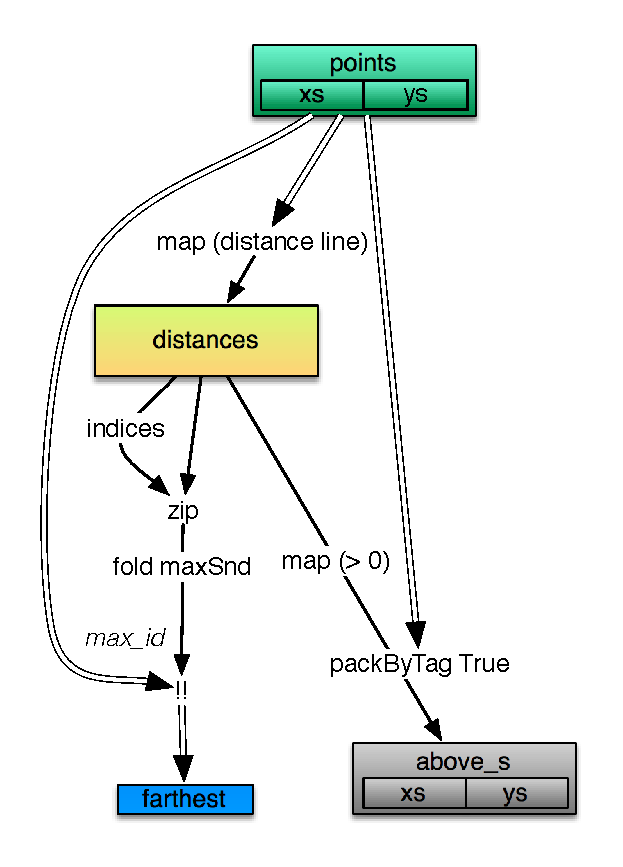
\includegraphics[width=0.4\textwidth,center]{img/QuickHull-flat-but-true}

\caption{\label{fig:QHFlat}{AST for the core of QuickHull example: arrow labels are AST nodes, coloured boxes are potentially manifest arrays.}}
\end{figure}

The above example uses six array combinators: @map@, @zip@, @indices@, @pack@, @fold@ and the indexing combinator @(!!)@. The first four of them are \*array transducers* in that they both consume and produce arrays. On the other hand @fold@ and @(!!)@ consume arrays and return a scalar value, so we call them pure consumers.

It is now time to show the AST node constructors these combinators correspond to. LiveFusion AST is a Generalised Algebraic Data Type (GADT) \todo{ref} whose individual constructors correspond to delayed array operations. In principle, given an interpreting function such as @eval :: AST t -> t@ an value of type @t@ encoded in the @AST@ language can be computed. Nowhere does it specify that @t@ is an array. In fact we know not all of the array combinators return an array: it has been discussed that @fold@, @(!!)@ and several others return a scalar value. To express the dimensionality of the result we introduce @type ArrData a@ which in our implementation is represented by @Vector a@ from @vector@ package \todo{ref}. We introduce type synonyms @ArrayAST a@ and @ScalarAST a@ to distinguish between the two.

\begin{lstlisting}[basicstyle={\ttfamily},language=Haskell]
type ArrayAST a = AST (ArrData a)
type ScalarAST a = AST a

data AST t where
  Map      :: (Elt a, Elt b)
           => Exp (a -> b)
           -> ArrayAST a
           -> ArrayAST b

  Zip      :: (Elt a, Elt b)
           -> ArrayAST a
           -> ArrayAST b
           -> ArrayAST (a,b)

  Fold     :: Elt a
           => Exp (a -> a -> a)
           -> ScalarAST a
           -> ArrayAST a
           -> ScalarAST a

  PackByTag :: Elt a
            => ArrayAST Bool
            -> ArrayAST a
            -> ArrayAST a

  Indices  :: Elt a
           => ArrayAST a
           => ArrayAST Int

  Index    :: Elt a
           -> ArrayAST a
           -> ArrayAST Int
           -> ScalarAST a
\end{lstlisting}



\section{Parametrising higher-order functions}

Another notable feature of the interface to note here is the type of functions parametrising the higher-order combinators like @map@ and @fold@. They are all of the form @Exp (a -> b)@ or @Exp (a -> a -> b)@. The corresponding functions in Haskell Prelude or array libraries like @Vector@ or @Repa@ accept as arguments simple Haskell functions like @a -> b@ or @a -> a -> a@ as long as the types match. So why cannot LiveFusion be the same? The answer lies in the approach to evaluating the AST. LiveFusion AST is open to interpretation by several backends as discussed in Section \todo{ref}, and the currently supported one includes the compilation step. When using this backend, the AST is compiled to one or more loops for which Haskell code is generated and written out to file. If the parametrising functions were simple Haskell functions, they would have be compiled to machine code before the program is run. When the AST is later constructed at runtime they would only be available in form of closures which can be called but not inspected\footnote{There is a non-portable way to explore closures in Haskell, but it will not allow one to easily make use of the code compiled to binary. See discussion in Section \todo{ref}}. Suppose the user calls @map (+1) xs@. The mentioned array libraries rely on the function @(+1)@ being inlined into the compiled loop code to produce efficient code. If this does not happen, calling @(+1)@ for every element in the array will result in the following:
\begin{enumerate}
\item Boxing the element value by placing it in the heap
\item Calling the closure with the pointer to the boxed value
\item Jumping to the address of the @(+1)@ function referenced in the closure
\item The code will unbox the value, increment it and create a new value on the heap
\item The loop code will then need to unbox the result and write it into the result array
\end{enumerate}

This is a very round-about way of incrementing a value in a tight loop and will greatly affect the performance of the loop. Unfortunately, at the time of generating code for AST, all these Haskell functions will have been compiled to machine code and are only available as closures. There is currently no way to inline them or get the original Haskell source code from which they were created. We needed to find a way to generate efficient code for user specified functions at runtime.

Thus, we need a way to record the user-provided functions in a more high level way than machine code. In summary our representation for functions:
\begin{enumerate}
\item Provides backend independent interface offering many common functions
\item Allows backend-specific implementation for each function
\item Hides implementation from the user by default
\item Allows user to compose functions in a way that looks very native
\item Allows user to provide direct backend-specific implementation for new functions that cannon be composed from functions already provided
\end{enumerate}

%% Does Accelerate fix the primitive functions as constructors in an ADT?

So what is @Exp (a -> b)@? It is a term in our scalar expression language $Exp$, representing a function from type $a$ to type $b$:
\begin{lstlisting}[basicstyle={\ttfamily},language=Haskell]
data Exp t where
  -- Literal or non-function value
  ConstE :: a -> Exp a

  -- Function implemented in the backend
  FunE :: Impl t -> Exp t

  -- Lambda abstraction
  LamE :: (Exp s -> Exp t) -> Exp (s -> t)

  -- Function application
  AppE :: Term (s -> t) -> Term s -> Term t
\end{lstlisting}

\todo{discuss HOAS and distinction between function values and non function values}

\todo{discuss Exp and HOAS, for now skipping to Impl}

The notable part of the @Exp@ language is its constructor @FunE@. The only argument to the constructor is @Impl t@ which is a backend-dependent way of defining a function. @Impl@ gives freedom to the backend to choose the most suitable representation for a function. For instance, in out Haskell backend, we are interested in generating Haskell source code, for which \name{Template Haskell} \todo{ref} is a natural choice. Thus we choose the following definition of @Impl@:
\begin{lstlisting}[basicstyle={\ttfamily},language=Haskell]
data Impl t = HsImpl {
                hs :: t,        -- Native Haskell function
                th :: Q TH.Exp  -- TemplateHaskell quasiquoted expression
              } 
\end{lstlisting}

The Template Haskell expression is really the core part of the function representation, but this is what would later on allow us to produce Haskell source code without much trouble. We also include simple Haskell function with our representation. At present this is just for completeness. However in the future it may be possible to avoid compiling certain parts of AST at runtime and run statically scheduled combinators. In this case this would be the function to inline in the loop.

We will now show the (rather trivial) implementations for a couple of functions before continuing with our explanation of Impl.

\begin{lstlisting}[basicstyle={\ttfamily},language=Haskell]
plusImpl :: Num a => Impl (a -> a -> a)
plusImpl = HsImpl { hs = (+); th = [| (+) |] } 

absImpl :: Num a => Impl (a -> a)
absImpl = HsImpl { hs = abs; th = [| abs |] } 
\end{lstlisting}

It is easy to see that TemplateHaskell expressions are trivially created from simple Haskell functions using QuasiQuotation syntax \todo{ref}. When the backend is ready to generate Haskell source for these functions, it will be a simple matter of using a pretty printer. The reasons for using TemplateHaskell instead of strings in the first place when the conversion is so trivial are the following:
\begin{itemize}
\item The backend does more than trivial code generation as discussed in Section \todo{ref}, where the full power of TemplateHaskell is required. Functions defined via TemplateHaskells become very easy to incorporate into the syntax tree being generated
\item New developments in TemplateHaskell\footnote{Starting with GHC 7.8.} will allow its expressions to be typed. Having @Q (TExp t)@ as opposed to @Q Exp@ will provide an extra layer of safety to our function representation
\end{itemize}


\section{On the flexibility of parametrising functions}

\begin{itemize}
\item Currently function representation of only one backend was shown, namely Haskell source backend.
\item Even that one was trivial: only containing a TH Exp + native HS function
\item What other functionality may we want in our function representation?
\item LiveFusion is a fast array processing library. The focus is on performance.
\item Our two main options for speed on modern CPUs: parallelism + vector instructions.
\item Parallelism is already exploited by DPH through other means and will split the computations evenly across all cores
\item Vectorisation on the other hand has not been exploited by DPH yet\footnote{Though new developments in that area have emerged more recently \todo{ref}}
\item The CPU manufacturers are introducing and announcing more and more vector instruction sets \footnote{\todo{ref}: Intel Future Instruction Sets} which will allow many types of vector operations to be performed on each core.
\item This is very handy for libraries like LiveFusion which are already providing patterns of array computation, some of which map very well to vector instructions of current or future CPUs \todo{find examples, but this will definitely include point-wise arithmetic, reductions and pack}.
\item At some point in the future @Impl@ function representation may be the most natural place to include backend- or even CPU-specific information, on how to generate vector instructions for a particular function, e.g. a reduction using product operator on an Intel CPU.
\end{itemize}

\section{Userland implementation of parametrising functions}

One feature of the given scalar functions representation allows the user to provide implementation of arbitrary functions the way they want the backend to generate them. After all, it only requires creating a new record of type @Impl t@ where @t@ is the type of the desired function. Library user can then provide the internals of function implementation to appear in the generated code.

This functionality may seem unnecessary, since the library already provides all functions from such type classes as @Num@, @Ord@, @Floating@, etc., as well as a powerful mechanisms to compose them into more complex functions. However, in the light of vector instructions discussion in Section \todo{ref}, leaving this door open to the user may be valuable and make the library more flexible on more architectures.


\clearpage

\section{Compiling Delayed LiveFusion AST}

\section{Sharing recovery: Abstract Semantic Graphs}

\begin{itemize}
\item Begin with Oleg's blessing quote. On two probs.
\item Find example, should be plenty in QuickHull
\item Talk about ref transparency of Haskell
\item Two types of sharing really, talk shapes
\item While can still fuse, it performs unnecessary work
\item Implicit vs. explicit sharing (ref email thread)
\item For implicit:
\item Still represented by the same object internally at runtime
\item StableNames, Gill's, but can do other, pointer equality sharing recovery
\item It's is IO, but since we are in a library and can guaranty safety by design we don't care
\end{itemize}


\IfNotCompilingAll{\bibliography{bib}}

\end{document}